\documentclass[conference]{IEEEtran}
\IEEEoverridecommandlockouts
% The preceding line is only needed to identify funding in the first footnote. If that is unneeded, please comment it out.
\usepackage{cite}
\usepackage{amsmath,amssymb,amsfonts}
\usepackage{algorithmic}
\usepackage{graphicx}
\usepackage{textcomp}
\usepackage{xcolor}
\usepackage{tikz}
\usepackage{hyperref}
\def\BibTeX{{\rm B\kern-.05em{\sc i\kern-.025em b}\kern-.08em
    T\kern-.1667em\lower.7ex\hbox{E}\kern-.125emX}}
\begin{document}

\title{Addressing the Impact of Localized Training Data in Graph Neural Networks\\
	{%\footnotesize \textsuperscript{*}Note: Sub-titles are not captured in Xplore andshould not be used
	}
	%\thanks{Identify applicable funding agency here. If none, delete this.}
}

\author{\IEEEauthorblockN{Akansha}
	\IEEEauthorblockA{\textit{Department of Mathematics}\\
		\textit{Manipal Institute of Technology}\\
		Manipal Academy of Higher Education - 576104, India.\\
		akansha.agrawal@manipal.edu.}
	%\and
	%\IEEEauthorblockN{2\textsuperscript{nd} Given Name Surname}
	%\IEEEauthorblockA{\textit{dept. name of organization (of Aff.)}\\
		%\textit{name of organization (of Aff.)}\\
		%City, Country \\
		%email address or ORCID}
	%\and
	%\IEEEauthorblockN{3\textsuperscript{rd} Given Name Surname}
	%\IEEEauthorblockA{\textit{dept. name of organization (of Aff.)} \\
		%\textit{name of organization (of Aff.)}\\
		%City, Country \\
		%email address or ORCID}
	%\and
	%\IEEEauthorblockN{4\textsuperscript{th} Given Name Surname}
	%\IEEEauthorblockA{\textit{dept. name of organization (of Aff.)} \\
		%\textit{name of organization (of Aff.)}\\
		%City, Country \\
		%email address or ORCID}
	%\and
	%\IEEEauthorblockN{5\textsuperscript{th} Given Name Surname}
	%\IEEEauthorblockA{\textit{dept. name of organization (of Aff.)} \\
		%\textit{name of organization (of Aff.)}\\
		%City, Country \\
		%email address or ORCID}
	%\and
	%\IEEEauthorblockN{6\textsuperscript{th} Given Name Surname}
	%\IEEEauthorblockA{\textit{dept. name of organization (of Aff.)} \\
		%\textit{name of organization (of Aff.)}\\
		%City, Country \\
		%email address or ORCID}
}

\maketitle

\begin{abstract}
	Graph Neural Networks (GNNs) have achieved notable success in learning from graph-structured data, owing to their ability to capture intricate dependencies and relationships between nodes. They excel in various applications, including semi-supervised node classification, link prediction, and graph generation. However, it is important to acknowledge that the majority of state-of-the-art GNN models are built upon the assumption of an in-distribution setting, which hinders their performance on real-world graphs with dynamic structures. In this article, we aim to assess the impact of training GNNs on localized subsets of the graph. Such restricted training data may lead to a model that performs well in the specific region it was trained on but fails to generalize and make accurate predictions for the entire graph. In the context of graph-based semi-supervised learning (SSL), resource constraints often lead to scenarios where the dataset is large, but only a portion of it can be labeled, affecting the model's performance. This limitation affects tasks like anomaly detection or spam detection when labeling processes are biased or influenced by human subjectivity. To tackle the challenges posed by localized training data, we approach the problem as an out-of-distribution (OOD) data issue by by aligning the distributions between the training data, which represents a small portion of labeled data, and the graph inference process that involves making predictions for the entire graph. We propose a regularization method to minimize distributional discrepancies between localized training data and graph inference, improving model performance on OOD data. Extensive tests on popular GNN models show significant performance improvement on three citation GNN benchmark datasets. The regularization approach effectively enhances model adaptation and generalization, overcoming challenges posed by OOD data\footnote{Codes are available at \url{https://github.com/Akanshaaga/Reg_APPNP}.}.
	
	
	
	
	
	
	%Graph Neural Networks (GNNs) have emerged as a powerful framework for learning from and reasoning over graph-structured data. With the ability to capture complex dependencies and relationships between nodes, GNNs have achieved remarkable success in a wide range of applications. Despite the remarkable success of Graph Neural Networks (GNNs) in tasks such as node classification, link prediction, and graph generation, it is important to acknowledge that the majority of state-of-the-art GNN models are built upon the assumption of an in-distribution setting. However, in practice, it becomes challenging to meet this assumption when dealing with real-world graphs, such as social networks, citation networks, or population graphs. These graphs are often characterized by dynamic and evolving structures, diverse node attributes, and complex interactions. As a result, the performance of traditional GNN models tends to degrade when confronted with out-of-distribution (OOD) data. In this article, we aim to measure the impact of training the model on only a localized subset of the graph. This restricted training data may result in a model that performs well on the specific region it was trained on but fails to generalize and make accurate predictions for the entire graph. The inability of a GNN model trained on localized data to generalize effectively raises concerns in various domains. For instance, anomaly detection or spam detection tasks can suffer greatly when the labeling process is biased or influenced by human subjectivity. In such scenarios, the model's performance may be inflated within the labeled region, but its predictions outside that region may be erroneous. This limitation undermines the reliability and practical applicability of the GNN model. To tackle the challenges posed by localized training data, we approach the problem as an OOD data issue. We recognize the need to align the distributions between the training data, which represents a small portion of labeled data, and the graph inference process that involves making predictions for the entire graph. To bridge the gap between the localized training data and the whole-graph inference, we propose a regularization method. Our regularization approach focuses on minimizing the distributional discrepancy between the two distributions, ensuring that the model can accurately predict beyond the localized training subset. This regularization technique guides the model to adapt and generalize effectively, mitigating the limitations posed by localized training data. We conducted extensive tests on popular GNN models, applying our regularization strategy. The results showed a significant improvement in performance when handling OOD data. Specifically, we evaluated our approach on a well-known citation network and observed a 2$\%$ increase in accuracy compared to the previously reported results. These findings highlight the efficacy of our regularization method in enhancing model performance and addressing the challenges posed by OOD data.
\end{abstract}

\begin{IEEEkeywords}
	Graph neural networks (GNNs), Out-of-distribution (OOD) graph data, Semi-supervised learning, Distributional discrepancy in graph data
\end{IEEEkeywords}

\section{Introduction}
Graph Neural Networks (GNNs) have emerged as a powerful framework for learning from and reasoning over graph-structured data. With the ability to capture complex dependencies and relationships between nodes, GNNs have achieved remarkable success in a wide range of applications, including social network analysis \cite{fan-19a,dav_ajm-22a}, recommendation systems \cite{gao_wan-22a,chu_yao-22a,wan_yuy-22a}, drug discovery \cite{gau_day_jam-21a,pan_fer-22a,wie_koh-20a}, and knowledge graph reasoning \cite{yas_ren_bos-21a,ye_kum_sin-22a,zha_yao-22a}. GNNs are versatile and can be used for various tasks, such as graph generation, community detection, and anomaly detection. However, node classification \cite{xia_wan_dai-22a,oon_suz-19a}, link prediction and graph classification are some of the most prevalent and well-studied applications of GNNs.

Despite the remarkable success of Graph Neural Networks (GNNs) in tasks such as node classification, link prediction, and graph generation, it is important to acknowledge that the majority of state-of-the-art GNN models are built upon the assumption of an in-distribution setting\cite{kip_wel-2016a,vel_pet_gui-2017a,ham_wil_jur-2017a,wij_wan-19a}. In this scenario, the training and test data are assumed to be drawn from the same distribution. However, in practice, it becomes challenging to meet this assumption when dealing with real-world graphs, such as social networks, citation networks, or population graphs. These graphs are often characterized by dynamic and evolving structures, diverse node attributes, and complex interactions. As a result, the performance of traditional GNN models tends to degrade when confronted with out-of-distribution (OOD) data. 

Effectively handling OOD data is vital for ensuring the practical usability of GNNs in real-world scenarios with high-stakes applications. These applications include molecule prediction \cite{hu_fey_zit-20a}, financial analysis \cite{yan_zha_zho-21a}, criminal justice \cite{aga_lak_zit-21a}, autonomous driving \cite{lia_yan_hu-20a}, and pandemic prediction \cite{pan_nik_vaz-21a}. To address the OOD problem in GNNs, several attempts have made, for instance, data or graph augmentation \cite{yu_lia-23a, sui_wan_jia-22a, fen_wen_jie-20a}: these techniques involve introducing variations to the graph structure or node attributes during the training phase to simulate OOD scenarios. By training GNN models on augmented data that covers a broader range of graph variations, the models can learn to be more robust and generalize better to OOD data. Disentanglement-Based Graph Models \cite{li_hao_ziw-22a, fan_wan_mo-2022a, li_hao_ziw-21a, zho_kut_rib-22a}: this approach focuses on designing novel GNN architectures that explicitly disentangle the propagation step from the non-linear transformations. These models aim to separate the graph structure and the node attributes to better capture and model the complex relationships within the graph. Learning Strategies \cite{li_hao_ziw-22b, buf_dav_pie-22a, wu_boj_ale-22a, sad_ma_li-21a, fen_he_tan-19a, wan_li_jin-22a, liu_hu_wan-22a, liu_jin_pan-22a}: various learning strategies are proposed to improve GNN performance on OOD data. These strategies involve adapting the training process or loss functions to account for the challenges posed by OOD scenarios. 
%For instance, domain adaptation techniques, self-supervised learning, or incorporating external knowledge can be used to enhance GNNs' ability to generalize to OOD data by leveraging additional information or aligning the learned representations.

%By exploring these different avenues, researchers aim to develop GNN models that are more robust and effective in handling OOD data. These efforts involve augmenting data, developing disentanglement-based or causality-based graph models, and proposing novel learning strategies tailored to the specific challenges of OOD scenarios. These advancements contribute to bridging the gap between GNNs' performance on in-distribution and OOD data, facilitating their application in real-world graph analysis tasks.

In this article, we aim to measure the impact of training the model on only a localized subset of the graph. This restricted training data may result in a model that performs well on the specific region it was trained on but fails to generalize and make accurate predictions for the entire graph. The inability of a GNN model trained on localized data to generalize effectively raises concerns in various domains. For instance, anomaly detection or spam detection \cite{liu_che_yan-18a, wan_lin_cui-19a} tasks can suffer greatly when the labeling process is biased or influenced by human subjectivity. In such scenarios, the model's performance may be inflated within the labeled region, but its predictions outside that region may be erroneous. This limitation undermines the reliability and practical applicability of the GNN model. To tackle the challenges posed by localized training data, we approach the problem as an OOD data issue. We recognize the need to align the distributions between the training data, which represents a small portion of labeled data, and the graph inference process that involves making predictions for the entire graph. By minimizing the distributional shift between these two components, we aim to enhance the model's ability to generalize effectively and make accurate predictions beyond the limited training subset.

To bridge the gap between the localized training data and the whole-graph inference, we propose a regularization method. Our regularization approach focuses on minimizing the distributional discrepancy between the two distributions, ensuring that the model can accurately predict beyond the localized training subset. By simulating a shift in the training data, we introduce bias during the labeling process as done in \cite{zhu-21a}, creating a more significant difference between the two distributions. The regularization is then performed by minimizing the distributional discrepancy between the entire graph distribution and the training data distribution obtained with the introduced bias. This regularization technique guides the model to adapt and generalize effectively, mitigating the limitations posed by localized training data.

%Our empirical study shows that in general disentangled GNN models \cite{zhu-21a,gas_etal-19a,liu_gao_ji-20a} offer more promising solution for effectively addressing the challenge of OOD data, where the training data is localized while predictions are required for the entire graph than regular state-of-the-art models \cite{kip_wel-2016a,vel_pet_gui-2017a,ham_wil_jur-2017a}. 

\textbf{Key observation.} Our observations reveal that the degradation in accuracy in traditional state-of-the-art Graph Neural Networks (GNNs) \cite{kip_wel-2016a,vel_pet_gui-2017a,ham_wil_jur-2017a} can be attributed to the propagation of mismatched probability distributions. This issue becomes exacerbated with each layer, resulting in poor accuracy. Consequently, in the context of out-of-distribution (OOD) graph data, improving accuracy necessitates minimizing the discrepancy between domain-specific features before propagation in the classification task. In light of this, we find that models \cite{gas_etal-19a,liu_gao_ji-20a, fen_wen_jie-20a} which treat propagation and nonlinear transformation operations as separate steps tend to perform better on OOD graph data. 

\textbf{Our contributions.} Our contributions in this research are threefold. Firstly, the proposed technique demonstrates stability by consistently improving the average prediction accuracy while maintaining a small standard deviation. This indicates that our regularization method reliably enhances the model's performance on out-of-distribution (OOD) data. Secondly, the proposed regularization approach can be applied to any given graph or Graph Neural Network (GNN) model, making it a versatile solution for addressing OOD data challenges across various domains. Lastly, in the experimental section, we conducted extensive tests on popular GNN models, applying our regularization strategy. The results showed a significant improvement in performance when handling OOD data. Specifically, we evaluated our approach on a well-known citation network and observed a significant increase in accuracy compared to the previously reported results in \cite{zhu-21a}. These findings highlight the efficacy of our regularization method in enhancing model performance and addressing the challenges posed by OOD data.


\section{Related Work} 
%There are several techniques are proposed to tackle the problem of OOD in graph data which are mostly categorize in three category: data or graph augmentation techniques: these techniques involve introducing variations to the graph structure or node attributes during the training phase to simulate OOD scenarios. By training GNN models on augmented data that covers a broader range of graph variations, the models can learn to be more robust and generalize better to OOD data \cite{yu_lia-23a,sui_wan_jia-22a,fen_wen_jie-20a}, disentanglement and Causality-based graph neural networks: this approach focuses on designing novel GNN architectures that explicitly disentangle the propagation step from the non-linear transformations. These models aim to separate the graph structure and the node attributes to better capture and model the complex relationships within the graph \cite{li_hao_ziw-22a,fan_wan_mo-2022a,li_hao_ziw-21a,li_hao_ziw-22a,zho_kut_rib-22a}.  Learning Strategies: various learning strategies are proposed to improve GNN performance on OOD data. These strategies involve Graph Invariant Learning \cite{li_hao_ziw-22b, buf_dav_pie-22a,zhu-21a}, graph adversarial learning \cite{wu_boj_ale-22a,sad_ma_li-21a,fen_he_tan-19a} and Graph Self-supervised Learning \cite{wan_li_jin-22a,liu_hu_wan-22a,liu_jin_pan-22a}, adapting the training process or loss functions to account for the challenges posed by OOD scenarios.However, our work is closely follow the line of shift robust GNN and size shift regularization method \cite{zhu-21a,buf_dav_pie-22a}. 

Various techniques have been proposed to address the problem of out-of-distribution (OOD) data in graph-based scenarios. These techniques can be broadly categorized into three categories.

The first category involves data or graph augmentation techniques. These techniques introduce variations to the graph structure or node attributes during the training phase to simulate OOD scenarios. By training Graph Neural Network (GNN) models on augmented data that covers a broader range of graph variations, the models can learn to be more robust and generalize better to OOD data. Several studies have explored this approach and demonstrated its effectiveness \cite{yu_lia-23a, sui_wan_jia-22a, fen_wen_jie-20a}.

The second category focuses on disentanglement and causality-based GNNs. These approaches aim to design novel GNN architectures that explicitly separate the propagation step from the non-linear transformations. By disentangling the graph structure and node attributes, these models can better capture and model the complex relationships within the graph, leading to improved performance on OOD data \cite{li_hao_ziw-22a, fan_wan_mo-2022a, li_hao_ziw-21a, zho_kut_rib-22a}.

The third category comprises learning strategies specifically tailored for OOD scenarios. Various learning strategies have been proposed to enhance GNN performance on OOD data. These strategies include graph invariant learning, graph adversarial learning, and graph self-supervised learning. Graph invariant learning aims to learn representations that are invariant to graph isomorphisms, while graph adversarial learning focuses on training GNNs that are robust against adversarial attacks. Graph self-supervised learning leverages unlabeled data to pretrain GNN models and learn meaningful representations. These learning strategies adapt the training process or loss functions to address the challenges posed by OOD scenarios \cite{li_hao_ziw-22b, buf_dav_pie-22a, wu_boj_ale-22a, sad_ma_li-21a, fen_he_tan-19a, wan_li_jin-22a, liu_hu_wan-22a, liu_jin_pan-22a}.

However, our work closely follows the line of shift-robust GNNs and employs a size shift regularization method \cite{zhu-21a, buf_dav_pie-22a}. Inspired by these approaches, we aim to tackle the challenges of OOD data by introducing regularization that simulates a shift in the training data. Our regularization method is designed to make the model more robust to this shift and improve its performance on OOD data scenarios.

\section{Preliminaries}
\textbf{Notation.} In our notation, the graph is represented as $G = (V, E)$, where $|V| = n$ denotes the number of nodes and $|E| = m$ denotes the number of edges in the graph. Specifically, $V$ represents the set of nodes, and $E$ represents the set of edges in the graph. To denote the $1$-hop neighborhood of a node $u$ in the graph, we use $N_u \subset V$, which represents the set of nodes that are directly connected to node $u$ within one edge. Furthermore, $(u, v)$ is used to denote an edge between node $u$ and node $v$, indicating a connection between the two nodes in the graph. In the context of the graph, we employ the adjacency matrix $A \in \{0,1\}^{n \times n}$, where each entry in the matrix corresponds to the presence or absence of an edge between two nodes. A value of $1$ indicates the presence of an edge, while a value of $0$ indicates the absence of an edge. This matrix captures the initial features $x_u\in \mathbb{R}^d$ associated with each node $u\in V$ in the graph, allowing for the representation of various node attributes or properties. Additionally, we utilize the feature matrix $\textbf{X} \in \mathbb{R}^{n \times d}$, where $n$ represents the number of nodes and $d$ denotes the dimensionality of the feature vectors. 

\textbf{Biased data generation.} To investigate the impact of localized training data on the node classification task, it is necessary to generate biased training data with controllable bias. In order to achieve this, we utilize the personalized PageRank vector of each node, denoted as $\Pi = (I-(1-\alpha)\tilde{A})^{-1}$. Here, $\tilde{A} = D^{-\frac{1}{2}}(A+I)D^{-\frac{1}{2}}$ represents the normalized adjacency matrix, where $D = \sum_{i=1}^{n}a_{ii}$ is the degree matrix of $A+I = (a_{ij})$ \cite{gas_etal-19a}. Following the methodology described in \cite{zhu-21a}, we employ this personalized PageRank vector to generate biased training data.

\textbf{Central Moment Discrepancy.}  Central Moment Discrepancy (CMD) is a the metric measures the direct distance between two distributions $p$ and $q$ using their central moments, given by
$$d_{CMD}(p,q) = \dfrac{1}{|b-a|}\|E(p)-E(q)\|_2+\sum_{k=2}^{\infty}\|c_k(p)-c_k(q)\|_2,$$
where $a, b$ denotes the joint distribution support, $E(\cdot)$ is the expected values of the distributions and $c_k(\cdot)$ are their respective central moments, considering different orders $k$ of moments.

\textbf{Maximum Mean Discrepancy.} Maximum Mean Discrepancy (MMD) is a metric used to measure the difference between means of distributions in a high-dimensional feature space defined by a kernel function. It quantifies the dissimilarity between two probability distributions by comparing their expected values in the rich Hilbert space. The formula for MMD is:
$$d_{MMD}(p, q) = \|\mu_p - \mu_q\|_H,$$
where $p$ and $q$ are two probability distributions, $\mu_p$ and $\mu_q$ are their means in the Hilbert space $H$, and $\|\cdot\|_H$ represents the norm in that space.

\textbf{Graph Neural Network (GNN) Layer}:
A typical $l$-th layer of a Graph Neural Network can be defined as follows:
\begin{align*}
	h^{(l)}_u & = propagation\biggl\{x^{(l-1)}_u, \{x^{(l-1)}_v \mbox{ where } v \in N_u\}\biggr\}\\
	x^{(l)}_u &  = transformation\{(h^{(l-1)}_u)\},
\end{align*}
where $x_u^{(l)}$ represents the feature vector of node $u$ at layer $l$, and $x_u^{(0)}$ is the initial feature representation of node $u$. The propagation step updates $x_u^{(l)}$ based on feature vectors of neighboring nodes in $N_u$, and the transformation step further processes the updated feature vector $h_u^{(l)}$. The process is repeated for a total of $K$ layers, with $\textbf{X}^{(K)}$ representing the final node feature matrix used for classification, and $\textbf{X}^{(0)} = \textbf{X}$.

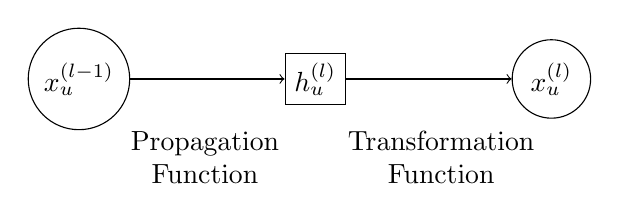
\begin{tikzpicture}[node distance=1cm, auto]
		% Nodes
		\node[draw, circle] (input) {$x^{(l-1)}_u$};
		\node[draw, rectangle, right of=input, xshift=2cm] (propagation) {$h^{(l)}_u$};
		\node[draw, circle, right of=propagation, xshift=2cm] (output) {$x^{(l)}_u$};
		
		% Arrows
		\draw[->] (input) -- (propagation);
		\draw[->] (propagation) -- (output);
%		\node (x1) at (0,0) {$x_1^{(0)}$};
%		\node (x2) [below of=x1] {$x_2^{(0)}$};
%		\node (x3) [below of=x2] {$x_3^{(0)}$};
%		\node (dots1) [below of=x3] {$\vdots$};
%		\node (xn) [below of=dots1] {$x_n^{(0)}$};
%		
%		\node (h1) [right of=x1, xshift=2cm] {$h_1^{(l)}$};
%		\node (h2) [right of=x2, xshift=2cm] {$h_2^{(l)}$};
%		\node (h3) [right of=x3, xshift=2cm] {$h_3^{(l)}$};
%		\node (dots2) [right of=dots1, xshift=2cm] {$\vdots$};
%		\node (hn) [right of=xn, xshift=2cm] {$h_n^{(l)}$};
%		
%		\node (xl) [right of=h3, xshift=2cm] {$x_3^{(l)}$};
%		
%		% Arrows
%		\draw[->] (x1) -- (h1);
%		\draw[->] (x2) -- (h2);
%		\draw[->] (x3) -- (h3);
%		\draw[->] (xn) -- (hn);
%		\draw[->] (h1) -- (xl);
%		\draw[->] (h2) -- (xl);
%		\draw[->] (h3) -- (xl);
%		\draw[->] (hn) -- (xl);
%		
%		% Dots
%		\draw[dotted] (dots1) -- (dots2);
		
		% Labels
		\node[align=center] at (1.6, -1) {Propagation\\Function};
		\node[align=center] at (4.6, -1) {Transformation\\Function};
		
	\end{tikzpicture}

%\textbf{Limitations.} The usual GNN models consists two major components: propagation and nonlinear transformation. Popular state-of-the-art GNN models, such as, graph convolution network (GCN) \cite{kip_wel-2016a} or graph attention networks (GAT) \cite{vel_pet_gui-2017a} may suffer from accuracy degradation when dealing with a large receptive field. It has been observed that these models tend to provide good accuracy only up to two layers. Several studies have revealed that increasing the number of layers in GCN can lead to a phenomenon known as over-smoothing \cite{li_han__wu-18a}. Researchers have explored the connection between GCN layers and random walks, demonstrating that stacking multiple layers can cause all node representations to become indistinguishable and converge to a stationary limit \cite{xu_li_tia_son-18a}. 

%Several works have been conducted to advance deep graph machine learning models that aim to capture information, particularly in scenarios with sparse and distributed labeled data across multi-hop neighborhoods, in order to achieve improved accuracy. Notable models in this direction include the Approximated Personalized Propagation of Neural Network (APPNP) \cite{gas_etal-19a} and the Deep Adaptive Graph Neural Networks (DAGNN) \cite{liu_gao_ji-20a}. APPNP treats prediction and propagation as two separate operations within a GNN model. Initially, the model predicts node labels based solely on the initial node features. Then, utilizing the concept of personalized PageRank (Page et al., 1999), the model performs neural prediction propagation. This personalized propagation operation helps refine and propagate the initial predictions throughout the graph, incorporating information from neighboring nodes. DAGNN takes a similar approach by employing a 2-layer Multilayer Perceptron (MLP) for the prediction task. After the initial prediction phase, DAGNN applies a propagation operation that introduces an adaptive mechanism to balance between local and global neighborhoods of the nodes. This adaptive mechanism enables the model to dynamically adjust the influence of local and global information, allowing it to capture both local node characteristics and global graph patterns.

%Our empirical study shows that in general aforementioned type of disentangled GNN models \cite{zhu-21a,gas_etal-19a,liu_gao_ji-20a} offer more promising solution for effectively addressing the challenge of OOD data, where the training data is localized while predictions are required for the entire graph than regular state-of-the-art models \cite{kip_wel-2016a,vel_pet_gui-2017a,ham_wil_jur-2017a}.



\section{Problem setup.}In this paper, we tackle the challenge of distributional shift in the context of semi-supervised learning (SSL) on a single graph where only a small portion is labeled. In traditional SSL, a common approach is to use the cross-entropy loss function, which calculates the difference between the predicted labels $\hat{y}_i$ generated by a graph neural network for each node $i$, and the true labels $y_i$. The overall loss $l$ is then computed as the average of individual losses over all training examples $M$:
\[ l = \frac{1}{M} \sum_{i=1}^{M} l(y_i, \hat{y}_i). \]

When training and testing data come from the same distribution, that is $P_{\text{train}}(X, Y) = P_{\text{test}}(X, Y)$, optimizing the cross-entropy loss on the training data ensures that the classifier is well-calibrated for making accurate predictions on the testing data. However, a significant challenge in machine learning arises when there is a mismatch between the distributions of the training and testing datasets, i.e., $P_{\text{train}}(X, Y) \neq P_{\text{test}}(X, Y)$. To address this issue, we focus on the distributional shift specifically in the output of the last hidden layer, which is denoted as $\hat{Y}$. Standard learning theory assumes that the distribution of labels given the representations $\hat{Y}$ is the same for both training and test data, that is $P_{\text{train}}(Y|\hat{Y}) = P_{\text{test}}(Y|\hat{Y})$.

% Figure environment removed

%To measure and mitigate this distributional shift, we use the Central Moment Discrepancy (CMD) as a distance metric. CMD quantifies the direct distance between two distributions $p$ and $q$ by comparing their central moments. The CMD formula involves calculating the difference between the expected values $E$ of the distributions and their respective central moments $c_k$, considering different orders $k$ of moments. In practice, a limited number of moments, such as up to the fifth order (k=5), are typically considered for efficiency.

%By utilizing CMD as a distance metric, we can effectively assess the discrepancy between distributions and evaluate the extent of the representation shift between the training and testing datasets in SSL tasks. This regularization technique enables the model to adapt and generalize more effectively, addressing the challenges posed by OOD data and improving the model's robustness in real-world scenarios.

\section{Regularized Approximate personalized propagation of neural prediction (Reg-APPNP)} In this section, we tackle the issue of distributional shift in graph neural networks, where the probability distributions of predicted labels differ between the training and testing data (i.e., $P_{train}(\hat{Y}) \neq P_{test}(\hat{Y})$). Since we have access to both the graph structure and unlabeled data, we propose a regularization technique that utilizes two discrepancy metrics: Central Moment Discrepancy (CMD) and Maximum Mean Discrepancy (MMD). These metrics allow us to quantify the dissimilarity between the probability distributions of the training and testing data.

\subsection{Reg-APPNP framework.}
We introduce our regularization method designed to minimize the discrepancy in the latent representations induced by distributional shift:
\begin{equation*}
	\begin{split}
		\mathcal{L}_{Reg-APPNP} = \dfrac{1}{M}\sum_{i=1}^{M}l(y_i,\hat{y}_i) + \lambda d_{CMD}(\hat{Y}_{train}, \hat{Y}_{test}) \\ +		
		\beta d_{MMD}(\hat{Y}{train}, \hat{Y}{test})
	\end{split}
\end{equation*}
In this formulation, the regularization term includes the cross-entropy loss (l) between true labels $y_i$ and predicted labels $hat{y}_i$, and two discrepancy metrics, CMD and MMD. The parameters $\lambda$ and $\beta$ control the importance of each regularization component. Empirical results demonstrate that incorporating both CMD and MMD metrics as regularization techniques potentially enhances the regularization's effectiveness because they capture different aspects of distributional shift. CMD assesses the direct distance between distributions, focusing on their central moments that convey shape and variability information. On the other hand, MMD emphasizes differences in the means of distributions, capturing more global distinctions.
%By combining CMD and MMD, we leverage their respective strengths to address distributional shift comprehensively. CMD's local focus captures fine-grained details, while MMD's global perspective handles overall distributional patterns.
Our approach employs the APPNP model \cite{gas_etal-19a} on biased data with the proposed regularization term. Extensive experiments on real-world citation networks reveal that in some cases, one metric may dominate in capturing distributional shift, while in others, both metrics contribute equally. We fine-tune the parameters $\lambda$ and $\beta$ to achieve improved accuracy in the semi-supervised learning (SSL) classification task.
\section{Experiments.}
In this section, we apply our proposed regularization technique to biased sample data, as generated in the work of Zhu et al. \cite{zhu-21a}. We use the same validation and test splits as in the GCN paper by Kipf and Welling \cite{kip_wel-2016a}. Our goal is to evaluate the effectiveness of our framework, Reg-APPNP, in minimizing distributional shifts compared to other baseline methods. Furthermore, we present a comprehensive study on hyperparameter optimization specifically for the CORA dataset. Hyperparameters play a crucial role in the performance of our regularization technique, and we thoroughly investigate and optimize these parameters to achieve the best results.

\textbf{Datasets.} In our experiments, we focus on the semi-supervised node classification task using three widely-used benchmark datasets: Cora, Citeseer, and Pubmed. For the biased training samples, we utilize the same data as generated for SR-GNN in Zhu et al.'s work \cite{zhu-21a}. To ensure fair comparison, we adopt the validation and test splits used in the GCN paper by Kipf and Welling \cite{kip_wel-2016a}. In order to obtain unbiased data, we perform random sampling from the remaining nodes after excluding those assigned to the validation and test sets.

\textbf{Baselines.} To investigate the performance under distributional shift, we employ two types of GNN models. Firstly, we utilize traditional GNNs that incorporate message passing and transformation operations, including GCN \cite{kip_wel-2016a}, GAT \cite{vel_pet_gui-2017a}, and GraphSage \cite{ham_wil_jur-2017a}. Secondly, we explore another branch of GNNs that treats message passing and nonlinear transformation as separate operations. This includes models such as APPNP \cite{gas_etal-19a} and DAGNN \cite{liu_gao_ji-20a}.

\textbf{Our Method.} Unless specified otherwise, we consider the instance of APPNP \cite{gas_etal-19a} with our proposed regularization technique, referred to as Reg-APPNP, as our base model. Additionally, we provide two ablations of Reg-APPNP for validation purposes. The first ablation includes only the CMD metric as regularization, and the second ablation includes only the MMD metric. By conducting these ablations, we aim to assess the effectiveness of our proposed Reg-APPNP method in addressing distributional shifts and enhancing the performance of the graph neural network models.

\textbf{Hyperparameters.}The primary parameters in our methods are the penalty parameters $\lambda$ and $\beta$, which correspond to the regularization metrics $d_{CMD}$ and $d_{MMD}$, respectively. Based on empirical results, we have determined the optimal values for these parameters for the SSL classification task on the three benchmark datasets. For the Cora dataset, we found that $\lambda = 0.5$ and $\beta = 1$ achieve the highest accuracy. In the case of Citeseer, the optimal values are $\lambda = 0.1$ and $\beta = 1$ , while for the Pubmed dataset, $\lambda = 0.1$ and $\beta = 0.1$ yield the best performance. Regarding the APPNP model, we set $\alpha = 0.1$, and we utilize the DGL (Deep Graph Library) layer for implementing the APPNP model within our experimental setup.  The results, including the impact of different values of $\lambda$ on the Cora dataset, are depicted in Figure \ref{fig:lambda_parameter}.
% Figure environment removed
\subsection{Experimental Results} We begin by presenting a performance comparison between our proposed regularization technique and the shift-robust technique proposed by Zhu et al. \cite{zhu-21a}, when combined with popular GNN models trained on biased training data. The F1-accuracy results for semi-supervised node classification for CORA data set are tabulated in Table \ref{table:reg_vs_sr}. The table demonstrates that our regularization technique consistently enhances the performance of each GNN model when applied to biased data. Notably, our method, Reg-APPNP, outperforms other baselines, including SR-GNN, on biased training data. 

This comparison confirms the efficacy of our proposed regularization technique in mitigating the impact of distributional shifts, leading to enhanced performance across various GNN models. Reg-APPNP emerges as the top-performing method, showcasing its effectiveness in handling biased training data and improving the accuracy of the semi-supervised node classification task.
\begin{table}[ht]
	\centering
	\caption{Performance comparison of our proposed regularization technique when combined with popular GNN models. The $F_1$-micro accuracy is reported and compared with the Shift-robust technique \cite{zhu-21a}.}
	\label{table:reg_vs_sr}
	\begin{tabular}{llll}
\hline \\[-0.7em]
Model & $F_1$-score & $F_1$-score w. Reg & $F_1$-score w. SR
\\\hline\\[-0.7em] \vspace{.1cm}
GCN & 65.35 $\pm$ $3.6$ & 71.41 $\pm$ $3.6$ & 70.45 $\pm$ $3.5$\\ \vspace{.1cm}
GraphSAGE & 67.56 $\pm$ $ 2.1$ & 72.10 $\pm $ $2.0$ & 71.79 $\pm $ $2.4$\\ \vspace{.1cm}
\textbf{APPNP} & 70.7 $\pm$ $ 1.9$  & \textbf{75.14 $\pm$ $1.8$} & 72.33 $\pm$ $ 5.9$\\ \vspace{.1cm}
DAGNN & 71.74 $\pm$ $ 0.32$  & 72.71 $\pm$ $ 0.31$ & 71.79 $\pm$ $ 0.36$	\\\vspace{.1cm}
\textbf{SR-GNN} & 73.5 $\pm $ $3.3$ \textbf{(\cite{zhu-21a})} &70.21 $\pm $ $0.87$	& 70.42 $\pm$ $ 1.1$ \\
\hline
	\end{tabular}
\end{table}

In their work \cite{zhu-21a}, the authors demonstrated that as the level of bias increases, popular GNN models experience a decline in performance. In Figure \ref{fig:biasing_parameter}, we present the behavior of our Reg-APPNP model as we increase the bias in the training data. The results clearly show that our proposed regularization technique consistently improves the performance in the SSL node classification task compared to the baseline APPNP model trained on biased data. 

% Figure environment removed
We applied our Reg-APPNP method to three popular citation GNN benchmarks and report the $F_1$-micro accuracy in Table \ref{table:reg_appnp}. To assess the impact of biased training data, we compare each model with the baseline APPNP trained on in-distribution IID data. As shown in the second row of Table \ref{table:reg_appnp}, APPNP's performance drops significantly when trained on biased data.

However, our proposed Reg-APPNP demonstrates significant improvement in performance on biased data, outperforming SR-GNN \cite{zhu-21a} when we executed their code on our system. It's worth noting that the results for SR-GNN in the table differ from the reported ones for Citeseer and Pubmed. The values in the table correspond to the results we reproduced using their code on our personal system.

Finally, we observe that combining both metrics, $d_{CMD}$ and $d_{MMD}$, is more effective than using only one of them during the entropy loss step. This finding further highlights the benefits of our comprehensive regularization approach in addressing distributional shifts and improving the performance of graph neural networks on biased training data.



\begin{table}[ht]
	\centering
	\caption{Performance comparison of Reg-APPNP on citation network benchmarks. We report $F_1$-micro accuracy and compare with APPNP trained on in-distribution IID data.}
	\label{table:reg_appnp}
	\begin{tabular}{llll}
		\hline \\[-0.7em]
		Model & Cora & Citeseer & Pubmed \\\hline \\[-0.7em] \vspace{.1cm}
		APPNP (Unbiased) &85.09 $\pm$ $ 0.25$ &75.73 $\pm$ $ 0.30$ & 79.73 $\pm$ $ 0.31$\\\hline \\[-0.7em] \vspace{.1cm}
		APPNP & 70.7 $\pm$ $ 1.9$ & 60.78 $\pm$ $ 1.6$ & 53.42 $\pm$ $1.3$\\ \vspace{.1cm}
		Reg-APPNP w.o. CMD & 71.37 $\pm$ $ 1.2$ & 60.46 $\pm $ $1.9$ & 53.35 $\pm $ $1.0$\\ \vspace{.1cm}
		Reg-APPNP w.o. MMD & 75.03 $\pm$ $ 1.2$  & 62.72 $\pm$ $ 1.9$ &66.13 $\pm$ $ 1.2$ \\ \vspace{.1cm}
		Reg-APPNP(ours) & \textbf{75.14 $\pm$ $ 1.8$}  & \textbf{65.01 $\pm$ $ 2.0$} & \textbf{70.71 $\pm$ $ 2.9$}	\\\vspace{.1cm}
		{SR-GNN} & 73.5 $\pm $ $3.3$ &62.60 $\pm $ $0.6$	& 68.78 $\pm$ $ 2.2$ \\
		\hline
	\end{tabular}
\end{table}


\section{Conclusion} In this work, we observed that as the level of bias increases, popular GNN models experience a decline in performance. We emphasized that biased training data is prevalent in real-world scenarios, and it can arise due to several reasons, such as challenges in labeling a large volume of data, the application of various heuristics or inconsistent techniques for node selection during labeling, delayed label assignment, and other constraints inherent in real-world problems. To address this challenge, we incorporate CMD and MMD as regularization terms in the APPNP model. This regularization approach encourages the model to minimize the discrepancy in the latent representations induced by the distributional shift. The proposed regularization approach can be applied to any given graph or Graph Neural Network (GNN) model, making it a versatile solution for addressing such challenges across various domains. This flexibility allows researchers and practitioners to leverage our method to improve their models' performance and generalization capabilities when dealing with OOD scenarios.
%In  This regularization technique aims to improve the generalization and robustness of the graph neural network model in the presence of distributional shift.



\section*{Acknowledgment}
I would like to express my sincere gratitude to Karmvir Singh Phogat for the valuable insights and critical feedback on the research problem addressed in this article. The thoughtful comments greatly contributed to the improvement and clarity of this work.

\bibliographystyle{./IEEEtran}
\bibliography{./IEEEabrv,bibfile_GNN}
\end{document}
